%!TEX TS-program = xelatex
%!TEX encoding = UTF-8 Unicode
\documentclass[12pt, xcolor=dvipsnames]{beamer}
\definecolor{slight}{gray}{0.9}
\fboxsep=10pt
\usecolortheme[named=Royal Blue]{structure}
\useinnertheme{circles}
\usepackage[no-math]{fontspec}
\usepackage{xltxtra, xunicode}
\usepackage[utf8]{inputenc}
\usepackage{tikz}
%\usepackage[sc, osf]{mathpazo}
\usepackage[minionint, lf, mathtabular]{MinionPro}
\setmainfont[Mapping=tex-text]{Minion Web Pro}
\setsansfont[Mapping=tex-text]{Myriad Web Pro}
\setmonofont[Scale=MatchLowercase]{Source Code Pro}
\usefonttheme{professionalfonts}
%% 中文字配置
\usepackage[
CJKmath=true, indentfirst=false, PunctStyle={quanjiao},
CheckSingle=true, SlantFont, BoldFont
]{xeCJK}
\setCJKmainfont[Scale=0.9, BoldFont=Hiragino Mincho ProN W6]{Hiragino Mincho ProN W3}
%\setCJKmainfont[Scale=0.9, BoldFont=Noto Sans CJK JP Bold]{Noto Sans CJK JP Medium}
\setCJKsansfont[Scale=0.9, BoldFont=Hiragino Sans W6]{Hiragino Sans W4}
%\setCJKsansfont[Scale=0.9, BoldFont=Hiragino Sans CNS W6]{Hiragino Sans CNS W3}
%\setCJKsansfont[Scale=0.9, BoldFont=Hiragino Sans W7]{Hiragino Sans W4}
%\setCJKsansfont[Scale=0.9, BoldFont=Source Han Sans UI TC Bold]{Source Han Sans UI TC Regular}
%\setCJKsansfont[Scale=0.9, BoldFont=PingFang TC Semibold]{PingFang TC Regular}
\setCJKmonofont[Scale=0.9, BoldFont=Yuanti TC Regular]{Hiragino Maru Gothic ProN W4}
\usepackage{fancyvrb, attachfile2, pstricks}
\usepackage{graphicx}
\setbeamerfont{page number in head/foot}{size=\tiny}
\setbeamertemplate{footline}[frame number]
\usepackage{xmpmulti, booktabs, multicol}
\setbeamertemplate{navigation symbols}{}
\let\WriteBookmarks\relax
\usepackage{dcolumn}
\newcolumntype{.}[1]{D{.}{.}{#1}}
\newcolumntype{,}[1]{D{,}{,}{#1}}

\linespread{1.25}

\setbeamersize{text margin left=.8em, text margin right=.6em}

\makeatletter
\defbeamertemplate{itemize item}{mycircle}{\LARGE\raise-1.6pt\hbox{\textbullet}}
\makeatother

\setbeamertemplate{itemize item}[mycircle]
\setbeamertemplate{itemize subitem}[triangle]
\setlength\leftmargini{1.3em}
\setlength\leftmarginii{1em}


%\CTXFR
\title{\bf{\Huge {}\\[-2mm] Principles of Economics \\[2mm] Review Session}}
\author{{\Large 張耕齊\\[2mm] Keng-Chi Chang}}
\institute{{}\\[-7mm]\footnotesize\tt{<r03323070@ntu.edu.tw>}\\[2mm]}
\date{\large 2016.12.21}
\begin{document}
\fontsize{12}{14pt}\selectfont

\begin{frame}
\titlepage
\end{frame}





\begin{frame}
\frametitle{\bf Condorcet Paradox 孔多塞悖論}
\begin{itemize}
\item Marquis de Condorcet (1785), French philosopher
\item Individual preferences cannot transmit to collective preferences through voting
\[\mbox{Voter 1: }A\succ B \succ C\]\\[-8mm]
\[\mbox{Voter 2: }B\succ C \succ A\]\\[-8mm]
\[\mbox{Voter 3: }C\succ A \succ B\]\\[-8mm]
\[\mbox{Pairwise voting: }A\succ B,\; B \succ C, \; C\succ A\]
\item That is, collective preference through voting is not {\it transitive}: 
\[\mbox{If }A\succ B \mbox{ and } B \succ C, \mbox{we should have }A\succ C\]
\item Key: Individual preference here is not {\it single peaked}
\item Order of voting matters and may result in dishonest/strategic votes. This is why 召委 is popular. See example below
\end{itemize}
\end{frame}


\begin{frame}
\frametitle{\bf Order of Voting and Strategic Voting}
\small \textsf{\bfseries Final 2007 Essay Q5.} Three groups of people are jointly deciding Daiwan national status. Assume each group has the same amount of voters. Here are their preferences: 
\begin{center}
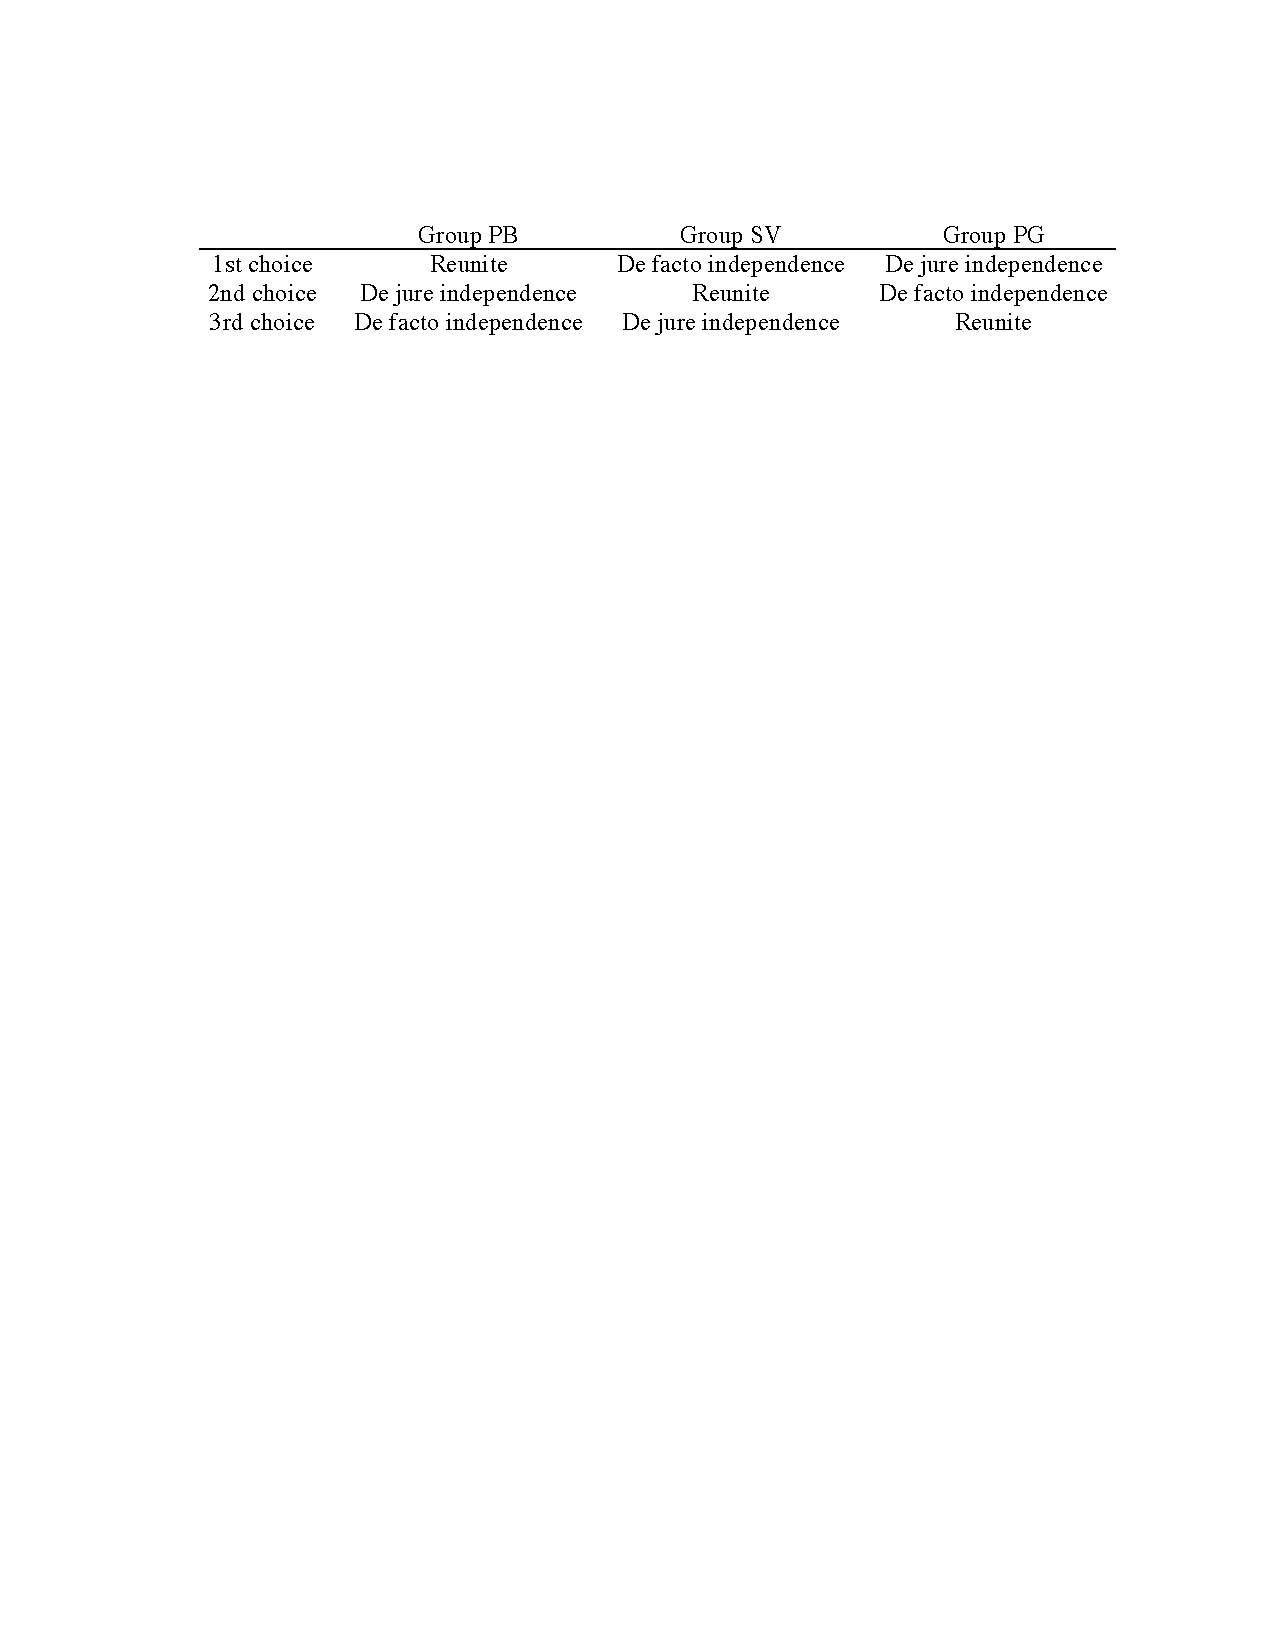
\includegraphics[width=.9\linewidth]{figures/q5.pdf}
\end{center}
\begin{enumerate}\itemsep-0.5ex 
\item[a.] Group PB suggests a vote by majority role. They propose that first they choose between de facto and de jure independence, and then choose between the winner of the first vote and reunite. If they all vote their preferences honestly, what outcome would occur?
\end{enumerate}
\end{frame}



\begin{frame}
\small 
\begin{center}
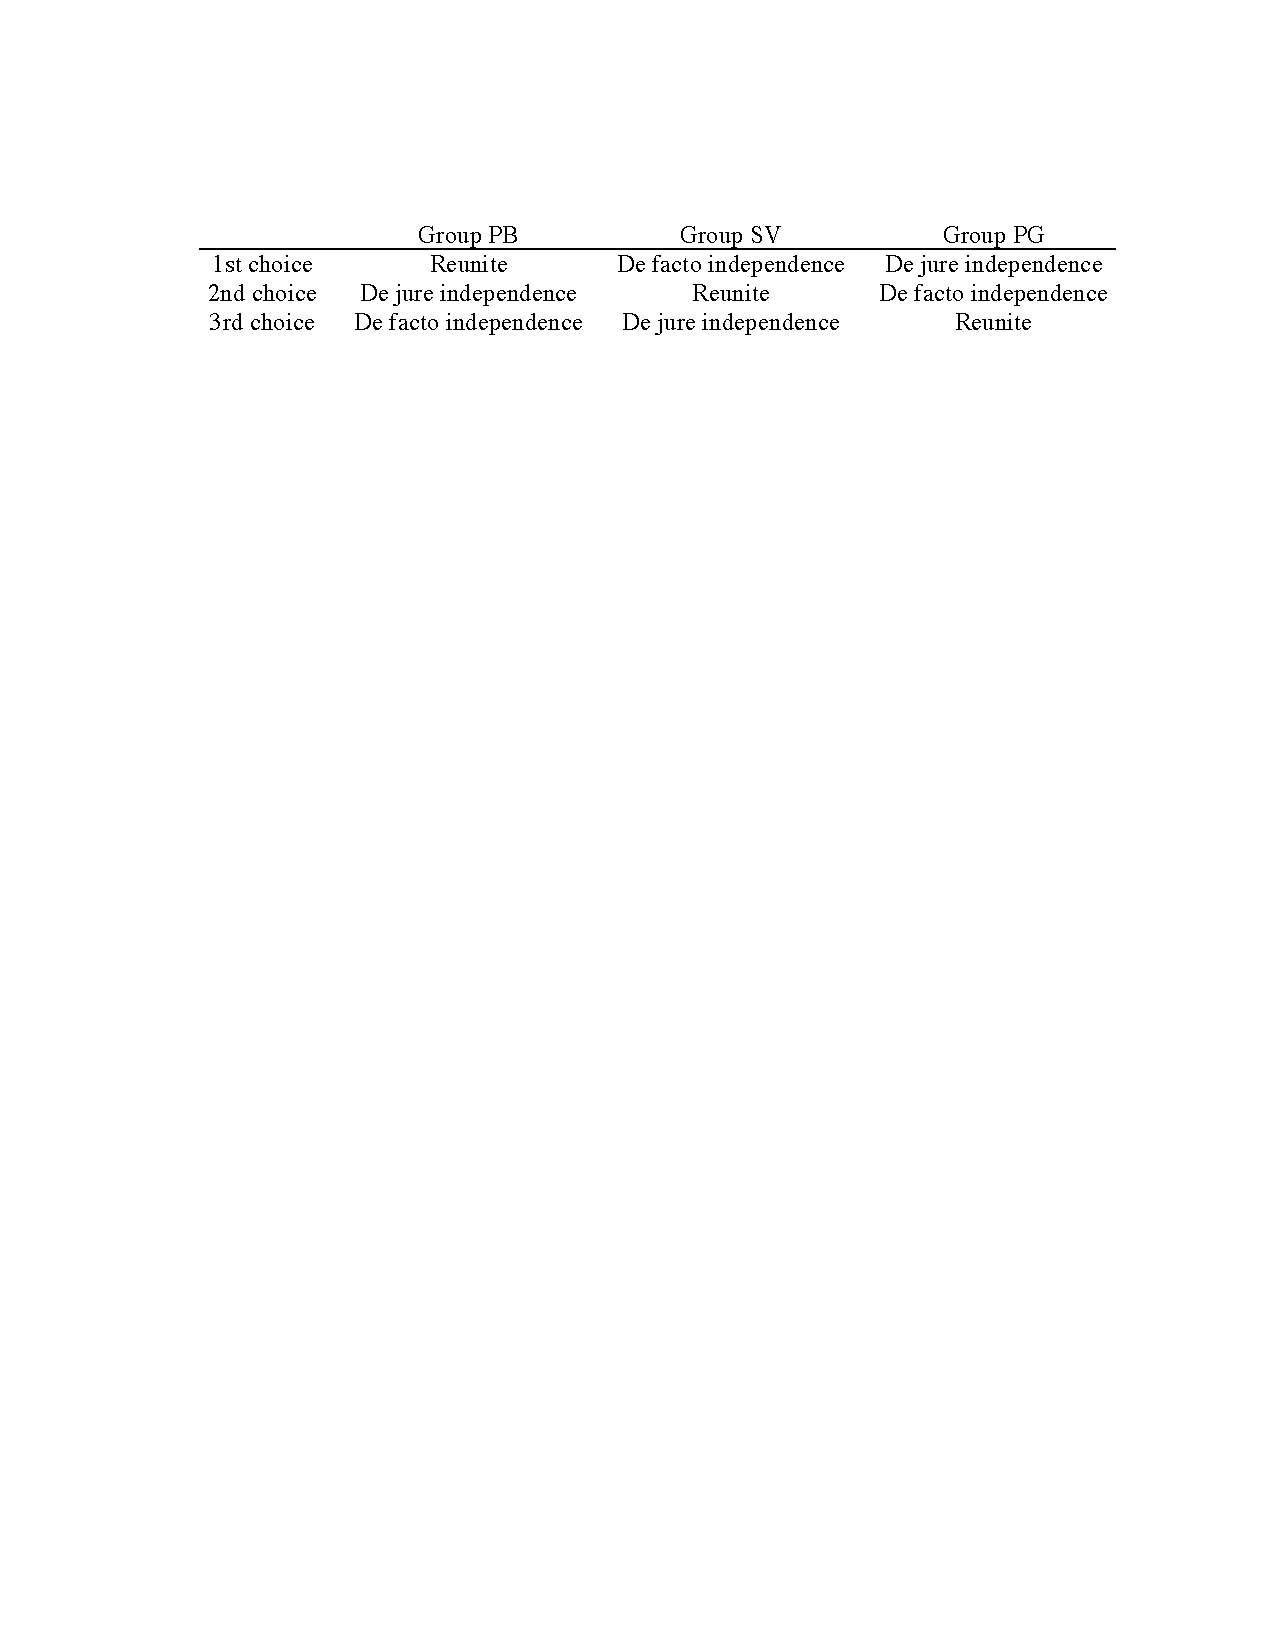
\includegraphics[width=.9\linewidth]{figures/q5.pdf}
\end{center}
\begin{enumerate}\itemsep-0.5ex 
\item[b.] Should group PG agree to group PB's suggestion? What alternative voting sequence would they prefer?
\item[c.] Group PB and SV convince group PG to go along with group PB’s voting system. In round one, group PG dishonestly says they prefer de facto independence over de jure independence. Why might they do this?
\item[d.] What standard property of decision making is violated here? 
\end{enumerate}
\end{frame}



\begin{frame}
\frametitle{\bf Arrow's Impossibility Theorem 不可能定理}
\begin{itemize}
\item Kenneth Arrow's 1950 PhD thesis, 1972 Nobel laureate for G. E.
\item There is {\it no} ideal voting scheme for aggregating individual preferences into a valid set of collective preferences
\item Three criteria for a good voting scheme: 
\begin{enumerate}
\item Unanimity 一致性: If everyone prefers $A$ to $B$, then $A$ should beat $B$
\item Transitivity 遞移性: If $A$ beats $B$, and $B$ beats $C$, then $A$ should beat $C$
\item Independence of irrelevant alternatives (IIA) 獨立性: Ranking between $A$ and $B$ should not depend on whether $C$ is available
\end{enumerate}
\item The only voting scheme that satisfies the above criteria is a dictatorship: Let someone make all the decision
\item Giving numerical representation to preferences (such as Borda Count, see example below) may preserve transitivity but fails independence of irrelevant alternatives
\end{itemize}
\end{frame}


\begin{frame}
\frametitle{\bf Borda Count is Transitive but Fails IIA}
\small \textsf{\bfseries ALL W3-5.} There is an alternative social decision method called a Borda Count. In this technique, alternatives are assigned a number based on the ranking of the alternatives by each agent. For example, suppose a society is trying to decide among four alternatives. If a voter likes alternative A better than any of the other three alternatives, A would receive a 4. If she likes C better than any of the remaining two alternatives, C would receive a 3. And so on. Suppose Adam, Bob, and Charlie are now voting on the issue of gun control. They are considering four alternatives:
\begin{enumerate}\itemsep-0.5ex 
\item Ban private ownership of guns entirely (B)
\item Severely restrict ownership of guns (S)
\item Moderately restrict ownership of guns (M)
\item Lightly restrict ownership of guns (L)
\end{enumerate}
\end{frame}


\begin{frame}
\small Here are the preferences of the three, from most preferred to least preferred:
\begin{center}
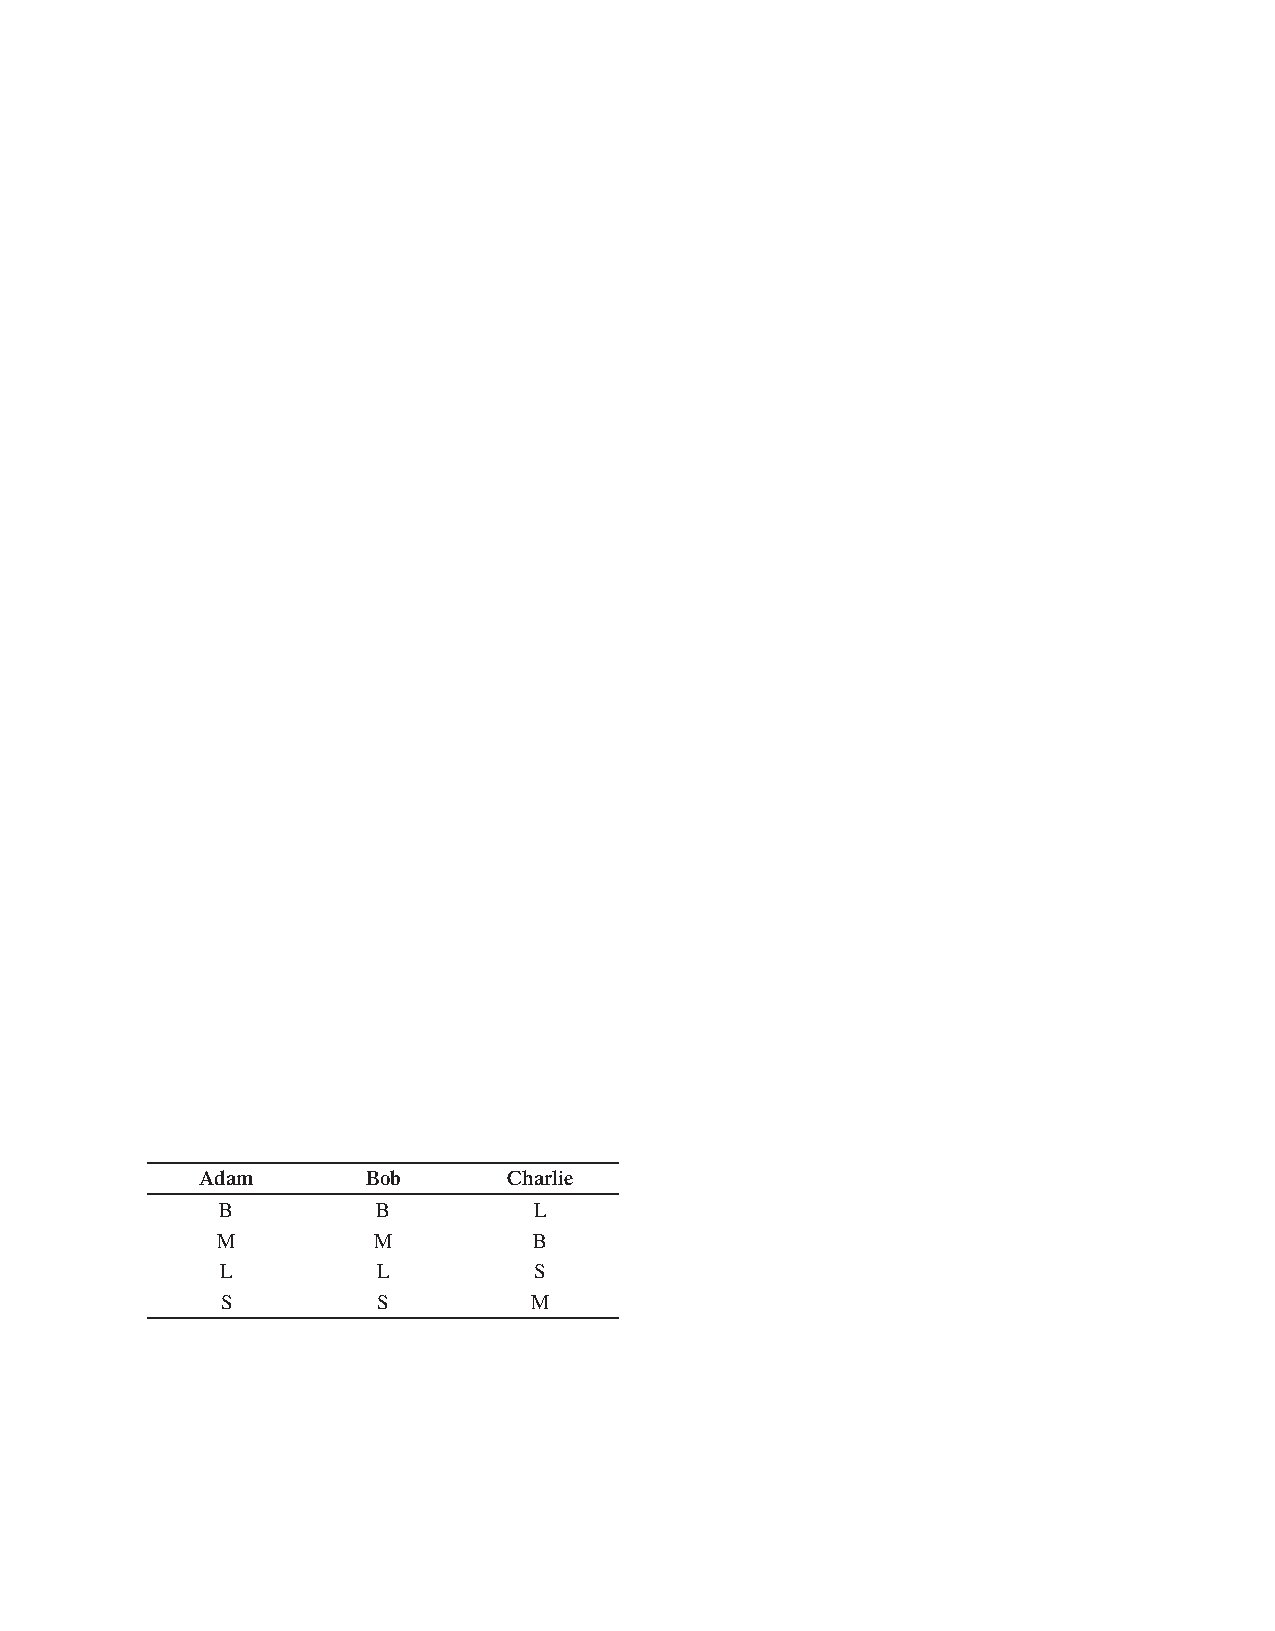
\includegraphics[width=.7\linewidth]{figures/w3-5.pdf}
\end{center}
\begin{enumerate}\itemsep-0.5ex 
\item[a.] Construct a Borda Count for the alternatives. What is the social ranking of the four based on the Borda Count?
\item[b.] Now assume the Supreme Court has ruled that bans and severe restrictions on guns are unconstitutional. So, neither B nor S is an option.
\end{enumerate}
\end{frame}


\begin{frame}
\frametitle{\bf Median Voter Theorem 中位選民定理}
\begin{itemize}
\item Harold Hotelling (1929, Arrow's adviser), Anthony Downs (1957)
\item Under single peaked preference, the desired policy of the {\it median voter} gets the majority vote
\[\mbox{Voter 1: }A\succ B \succ C\]\\[-9.5mm]
\[\mbox{Voter 2: }B\succ C \succ A\]\\[-8mm]
\[\mbox{Voter 3: }C\succ B \succ A\]\\[-8mm]
\[\mbox{Pairwise voting: }B\succ C \succ A\]
\item Voter 2 is the median voter and policy $B$ gets the majority vote
\item If there are enough competition and parties want to win, moving towards the center is a best response and endorsing the choice of the median voter is a Nash equilibrium
\item This makes parties looks similar and creates {\it policy convergence}
\end{itemize}
\end{frame}


\begin{frame}
\frametitle{\bf Why Democracy?}
\begin{itemize}
\item Democratic countries may have smaller mean in economic growth but also with a smaller variance, compare to monarchy or dictatorship. Slow but stable
\item Democratization may cause growth (Acemoglu et al. 2015)
\end{itemize}
\end{frame}

\begin{frame}
\begin{center}
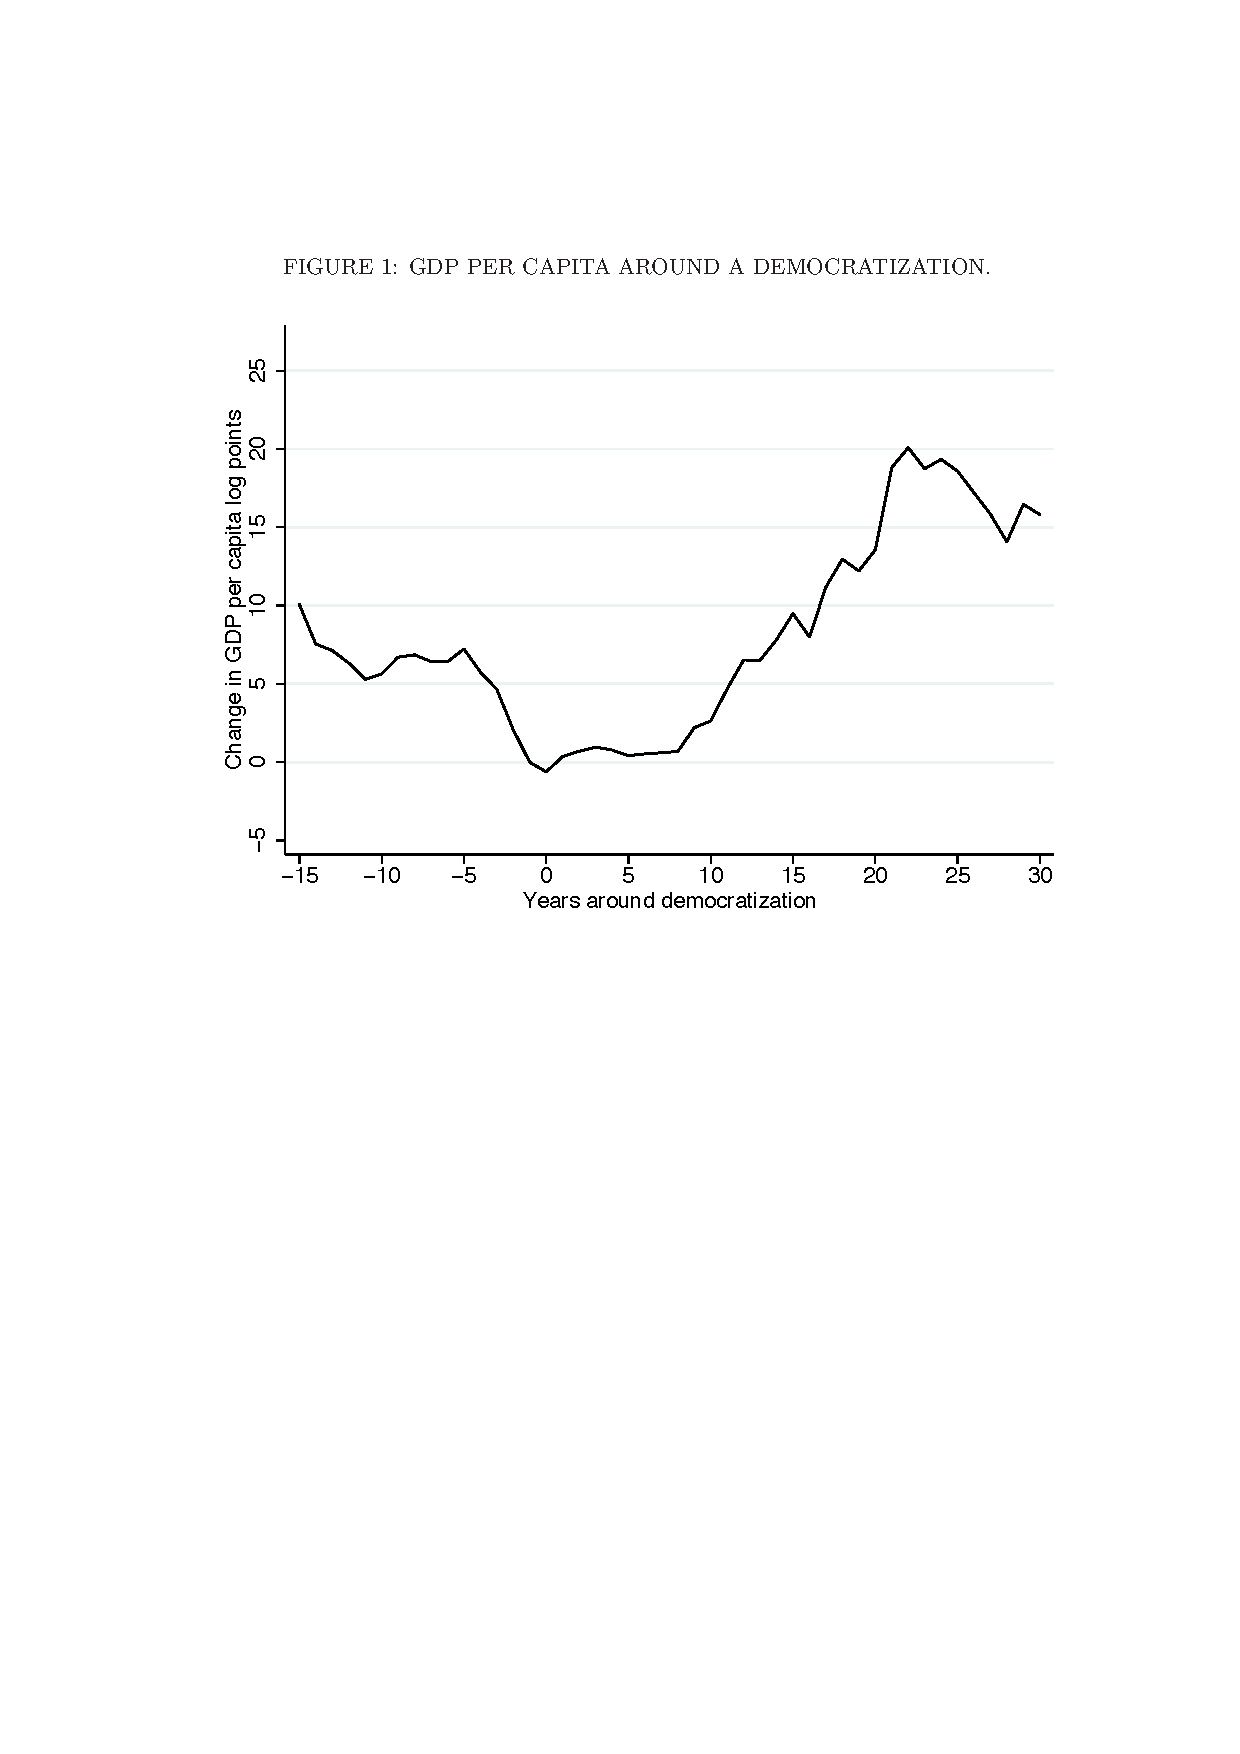
\includegraphics[width=.9\linewidth]{figures/growth.pdf}
\end{center}
\end{frame}


\end{document}